\begin{proposition}{Sine with Different Frequencies have the same Wave
Quality}{sine_with_different_frequencies_have_the_same_wave_quality}
    Any two waves given by \( \sin  \left( \alpha x \right) \) , \( \sin
    \left( \beta x \right) \) for \( \alpha , \beta  \in \mathbb{R} ^{ \neq 0 }
    \) have the same wave quality.
\end{proposition}
\begin{proof}
    Visually we can first see that:
    \begin{center}
        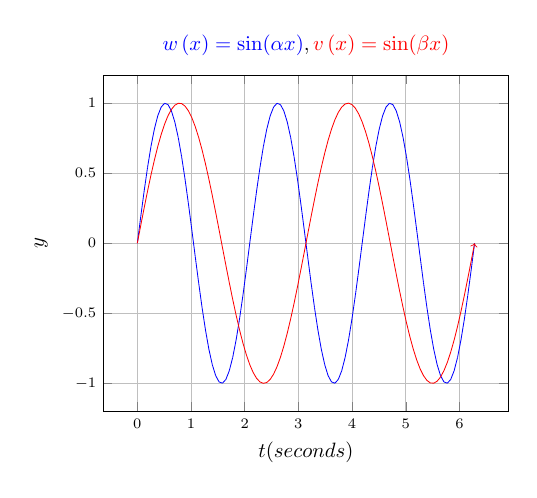
\begin{tikzpicture}[scale=.75]
          \begin{axis} [
              title = {$\textcolor{blue}{  w\left(x\right) = \sin(\alpha x)},
              \textcolor{red}{v\left(x\right) = \sin(\beta x)}$},
              xtick = {0,...,2 * pi},
              xlabel = $t (\text{seconds})$, ylabel = $y$,
              ticklabel style = {font = \scriptsize},
              grid
            ]
            \addplot [->, surf, domain=0:2 * pi , samples=100,blue, thin] { sin(3 * deg(x) ) };
            \addplot [->, domain=0:2 * pi , samples=100,red, thin] { sin(2 * deg(x) ) };
          \end{axis}
        \end{tikzpicture}
    \end{center}

    It's clear that one is a compression of the other, formally we can see that
    the red wave's period can be scaled by \( \frac{\alpha }{\beta } \) to
    become the blue wave.

  Notice that given a wave, and $ k \in \mathbb{R} ^{> 1}$ that $ u\left(kx\right)$ becomes compressed, and thus has a higher pitch.
\end{proof}
